\documentclass[11pt]{article}

\usepackage[a4paper,margin=1in]{geometry}
\usepackage{amsmath}
\usepackage{graphicx}
\usepackage{amssymb}
\usepackage{parskip}
\usepackage[table]{xcolor}
\usepackage{tikz}
\usetikzlibrary{arrows.meta, positioning, shapes.geometric, calc}
\usepackage[most]{tcolorbox}
\usepackage{titlesec}
\usepackage{enumitem}
\usepackage{booktabs}
\usepackage{array}
\usepackage{hyperref}

% ---------- Colors ----------
\definecolor{deepblue}{HTML}{1B3B6F}
\definecolor{accent}{HTML}{2E86AB}
\definecolor{accent2}{HTML}{E07A3F}
\definecolor{soft}{HTML}{F4F7FB}
\definecolor{soft2}{HTML}{FFF4EC}
\definecolor{linegray}{HTML}{D6DEE8}
\definecolor{textgray}{HTML}{333333}
\definecolor{codebg}{HTML}{1B3B6F}
\definecolor{codefg}{HTML}{F4F7FB}
\definecolor{greend}{HTML}{2E7D4F}
\definecolor{greensoft}{HTML}{EEF7F1}
\definecolor{pinkd}{HTML}{C2447A}
\definecolor{pinksoft}{HTML}{FDF0F6}
\definecolor{glossp}{HTML}{0F766E}
\definecolor{glosspsoft}{HTML}{F0FBFA}
\definecolor{glossgold}{HTML}{B45309}

% ---------- Section styling ----------
\titleformat{\section}
  {\Large\bfseries\color{deepblue}}
  {}{0em}{}[{\color{accent}\titlerule[1.2pt]}]
\titlespacing*{\section}{0pt}{18pt}{10pt}

\titleformat{\subsection}
  {\large\bfseries\color{accent}}
  {\thesubsection}{0.6em}{}
\titlespacing*{\subsection}{0pt}{14pt}{6pt}

% ---------- Reusable boxes ----------
\newtcolorbox{codebox}{
  colback=codebg, colframe=codebg,
  coltext=codefg,
  fonttitle=\bfseries,
  boxrule=0pt, arc=3pt, outer arc=3pt,
  left=8pt, right=8pt, top=6pt, bottom=6pt,
  fontupper=\ttfamily\small
}

\newtcolorbox{stepbox}[1]{
  colback=soft, colframe=deepblue,
  boxrule=0.8pt, arc=3pt, outer arc=3pt,
  left=10pt, right=10pt, top=6pt, bottom=6pt,
  title={#1}, fonttitle=\bfseries\color{white},
  colbacktitle=deepblue, coltitle=white
}

\newtcolorbox{plainbox}{
  colback=soft, colframe=accent,
  boxrule=0.8pt, arc=3pt, outer arc=3pt,
  left=10pt, right=10pt, top=6pt, bottom=6pt
}

\newtcolorbox{warnbox}{
  colback=soft2, colframe=accent2,
  boxrule=0.8pt, arc=3pt, outer arc=3pt,
  left=10pt, right=10pt, top=6pt, bottom=6pt
}

\newtcolorbox{greenbox}[1]{
  colback=greensoft, colframe=greend,
  boxrule=0.8pt, arc=3pt, outer arc=3pt,
  left=10pt, right=10pt, top=6pt, bottom=6pt,
  title={#1}, fonttitle=\bfseries\color{white},
  colbacktitle=greend, coltitle=white
}

\newtcolorbox{pinkbox}[1]{
  colback=pinksoft, colframe=pinkd,
  boxrule=0.8pt, arc=3pt, outer arc=3pt,
  left=10pt, right=10pt, top=6pt, bottom=6pt,
  title={#1}, fonttitle=\bfseries\color{white},
  colbacktitle=pinkd, coltitle=white
}

\newtcolorbox{glossarybox}[1]{
  enhanced,
  colback=glosspsoft, colframe=glossp,
  boxrule=0.9pt, arc=2pt, outer arc=2pt,
  left=16pt, right=16pt, top=8pt, bottom=10pt,
  title={#1}, fonttitle=\large\bfseries\color{white},
  colbacktitle=glossp,
  coltitle=white,
  width=0.62\textwidth
}

\newcommand{\glosslink}[2]{%
  \noindent{\color{glossgold}\textbullet}\;\,\textbf{\color{glossp}\hyperref[#2]{#1}}\\[6pt]
}

\hypersetup{
  colorlinks=true, linkcolor=deepblue, urlcolor=deepblue
}

\begin{document}

% ---------- Title ----------
\begin{center}
  {\Huge\bfseries\color{deepblue} A Simple Tutorial on\\[2pt] Few-Shot Learning}\\[4pt]
  {\color{accent}\rule{0.4\linewidth}{1pt}}
\end{center}
\vspace{8pt}

\begin{center}
\begin{glossarybox}{Terminology at a Glance}
\glosslink{Few-Shot Learning}{sec:whatisfewshot}
\glosslink{Zero-Shot Learning}{sec:zerooneshot}
\glosslink{One-Shot Learning}{sec:zerooneshot}
\glosslink{In-Context Learning}{sec:incontext}
\noindent{\color{glossgold}\textbullet}\;\,\textbf{\color{glossp}\hyperref[sec:fewshotprompting]{Few-Shot Prompting}}
\end{glossarybox}
\end{center}

\section*{What Is Few-Shot Learning?}
\phantomsection
\label{sec:whatisfewshot}

\textbf{Few-shot learning} means teaching a model to perform a task using only a \textbf{small number of examples}, rather than a large labeled dataset.

\begin{stepbox}{Example: Sentiment Classification}
\textbf{Example 1:}
\[
\text{``This movie was amazing.''} \rightarrow \text{Positive}
\]

\textbf{Example 2:}
\[
\text{``The movie was boring.''} \rightarrow \text{Negative}
\]

\textbf{Now classify:}
\[
\text{``I really enjoyed this film.''} \rightarrow \; ?
\]

\textbf{Expected answer:}
\[
\boxed{\text{Positive}}
\]
\end{stepbox}

%------------------------------------------------

\section*{Zero-Shot, One-Shot, and Few-Shot}
\phantomsection
\label{sec:zerooneshot}

These three settings differ only in \textbf{how many examples} are given to the model before it must answer.

\begin{stepbox}{Zero-Shot Example}
Instruction: \; \emph{Classify the sentiment of each review.}

Classify: \; \emph{``The food was excellent.''}

\vspace{4pt}
\textcolor{accent}{\textbf{Note:}} No prior examples are given — the model must rely only on the instruction itself.
\end{stepbox}

\begin{stepbox}{One-Shot Example}
Instruction: \; \emph{Classify the sentiment of each review.}

``The food was terrible.'' $\rightarrow$ Negative

Now: \; ``The food was excellent.'' $\rightarrow$ ?

\vspace{4pt}
\textcolor{accent}{\textbf{Note:}} A single labeled example is given before the new query.
\end{stepbox}

\begin{stepbox}{Few-Shot Example}
Instruction: \; \emph{Classify the sentiment of each review.}

``The food was terrible.'' $\rightarrow$ Negative

``The food was okay, nothing special.'' $\rightarrow$ Neutral

Now: \; ``The food was excellent.'' $\rightarrow$ ?

\vspace{4pt}
\textcolor{accent}{\textbf{Note:}} Several labeled examples are shown before the new query, giving the model a clearer sense of the pattern.
\end{stepbox}

%------------------------------------------------

\section*{Support Set and Query Set}

The \textbf{support set} is the small collection of labeled examples used to help the model understand or adapt to the task. The \textbf{query} is the new, unlabeled example the model must predict.

Consider an image classification task, where each item in the support set is an \emph{image} paired with its class label:

\[
\mathcal{S} = \big\{ (\text{cat}_1,\text{Cat}),\ (\text{cat}_2,\text{Cat}),\ (\text{dog}_1,\text{Dog}),\ (\text{dog}_2,\text{Dog}) \big\}
\]

\begin{center}
\resizebox{0.85\textwidth}{!}{%
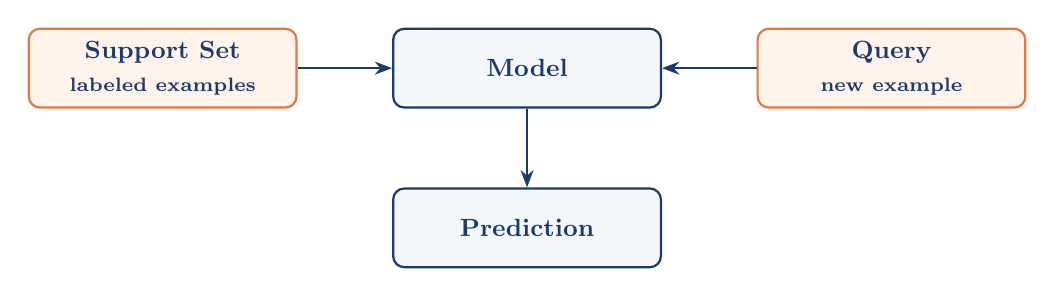
\begin{tikzpicture}[
  node distance=8mm and 12mm,
  box/.style={rectangle, rounded corners=4pt, draw=deepblue, thick,
              fill=soft, minimum width=34mm, minimum height=10mm,
              align=center, font=\small\bfseries\color{deepblue}},
  startbox/.style={box, fill=soft2, draw=accent2},
  arrow/.style={-{Stealth[length=2.2mm]}, thick, color=deepblue}
]
  \node[startbox] (support) {Support Set\\[1pt]\scriptsize labeled examples};
  \node[box, right=of support] (model) {Model};
  \node[startbox, right=of model] (query) {Query\\[1pt]\scriptsize new example};
  \node[box, below=10mm of model] (pred) {Prediction};

  \draw[arrow] (support) -- (model);
  \draw[arrow] (query) -- (model);
  \draw[arrow] (model) -- (pred);
\end{tikzpicture}%
}
\end{center}

%------------------------------------------------

\section*{$N$-Way $K$-Shot Learning}

Few-shot tasks are often described using the notation:

\[
\boxed{N\text{-way } K\text{-shot}}
\]

\begin{itemize}[leftmargin=1.4em, noitemsep]
  \item $N$ = number of classes in the task,
  \item $K$ = number of support examples given per class.
\end{itemize}

\begin{stepbox}{Example: 5-Way 2-Shot}
\[
5\text{-way } 2\text{-shot} \quad\Longrightarrow\quad 5 \text{ classes},\; 2 \text{ examples per class}
\]

The total size of the support set is:
\[
N \times K = 5 \times 2 = \boxed{10 \text{ examples}}
\]
\end{stepbox}

\begin{center}
\resizebox{0.8\textwidth}{!}{%
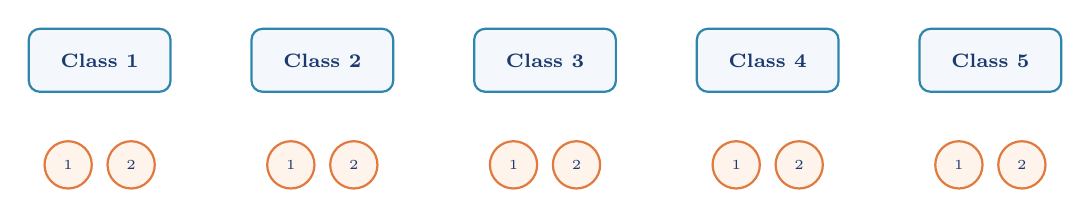
\begin{tikzpicture}[
  node distance=4mm and 10mm,
  cls/.style={rectangle, rounded corners=4pt, draw=accent, thick,
              fill=soft, minimum width=18mm, minimum height=8mm,
              align=center, font=\scriptsize\bfseries\color{deepblue}},
  ex/.style={circle, draw=accent2, thick, fill=soft2,
             minimum size=6mm, font=\tiny\color{deepblue}}
]
  \node[cls] (c1) {Class 1};
  \node[cls, right=of c1] (c2) {Class 2};
  \node[cls, right=of c2] (c3) {Class 3};
  \node[cls, right=of c3] (c4) {Class 4};
  \node[cls, right=of c4] (c5) {Class 5};

  \foreach \c/\name in {c1/c1,c2/c2,c3/c3,c4/c4,c5/c5} {
    \node[ex, below=6mm of \c, xshift=-4mm] {1};
    \node[ex, below=6mm of \c, xshift=4mm] {2};
  }
\end{tikzpicture}%
}
\end{center}

%------------------------------------------------

\section*{In-Context Learning}
\phantomsection
\label{sec:incontext}

For modern large language models, few-shot learning is usually done through \textbf{in-context learning}: the examples — often called \textbf{demonstrations} — are placed directly inside the prompt, and the model is not retrained. When this is done with several demonstrations, it is also called \textbf{few-shot prompting}.

\begin{codebox}
2 + 3 = 5\\
4 + 7 = 11\\
8 + 2 = ?
\end{codebox}

The model predicts $10$, simply by recognizing the pattern from the two demonstrations placed in the context.

\[
\boxed{\text{Prompt} = \text{Demonstrations} + \text{Query}}
\]

Crucially, the model's parameters are \textbf{not updated}.

%------------------------------------------------

\section*{Few-Shot Prompting vs.\ Few-Shot Fine-Tuning}
\phantomsection
\label{sec:fewshotprompting}

Two different ideas are sometimes both called \textbf{``few-shot learning.''} It is important to keep them separate.

\noindent
\begin{minipage}[t]{0.48\textwidth}
\begin{greenbox}{Few-Shot Prompting}
Examples are placed in the prompt:
\[
\text{Examples} + \text{Query} \rightarrow \text{Prediction}
\]
\centering \Large$\downarrow$\\[2pt]
\normalsize\textbf{No parameter update}
\end{greenbox}
\end{minipage}
\hfill
\begin{minipage}[t]{0.48\textwidth}
\begin{pinkbox}{Few-Shot Fine-Tuning}
Examples are used to actually train the model:
\[
\theta' = \theta - \eta \nabla_\theta L
\]
\centering \Large$\downarrow$\\[2pt]
\normalsize\textbf{Parameter update}
\end{pinkbox}
\end{minipage}

%------------------------------------------------

\section*{Example Selection in Few-Shot Prompting}

When many candidate examples are available but only a few can fit in the prompt, we must decide: \textbf{which examples should we select?}

\begin{stepbox}{Example: Relevance Matters}
Task: \; \emph{Classify the sentiment of each product review.}

Query:
\begin{quote}
\emph{``The battery lasts forever.''}
\end{quote}

More useful support example (topically related):
\begin{quote}
\emph{``The battery dies after one hour.''} $\rightarrow$ Negative
\end{quote}

Less useful support example (unrelated topic):
\begin{quote}
\emph{``The restaurant was terrible.''} $\rightarrow$ Negative
\end{quote}

The battery-related example is more useful because it is closer in topic and structure to the query.
\end{stepbox}

Good support examples should ideally be:

\begin{itemize}[leftmargin=1.4em, noitemsep]
  \item \textbf{relevant} to the query,
  \item \textbf{correctly labeled},
  \item \textbf{diverse}, covering different cases,
  \item \textbf{representative} of the overall task.
\end{itemize}

The \emph{order} in which examples are presented can also affect an LLM's predictions. Therefore, a core few-shot learning problem is to \textbf{select good examples} and \textbf{choose a good order}.

\begin{warnbox}
\textbf{More examples are not always better.} A small set of high-quality, relevant examples can outperform a larger set of noisy or poorly chosen ones.
\end{warnbox}

%------------------------------------------------

\section*{Few-Shot Prompting vs.\ RAG}

\textbf{Few-shot examples} show the model how to perform the task, while \textbf{RAG} provides the information needed to perform it.

\end{document}